\chapter{Data Exploration}
\label{chapter:data}
\section{EU-Forest Labels}

\begin{figure}[!thb]
    \centering
    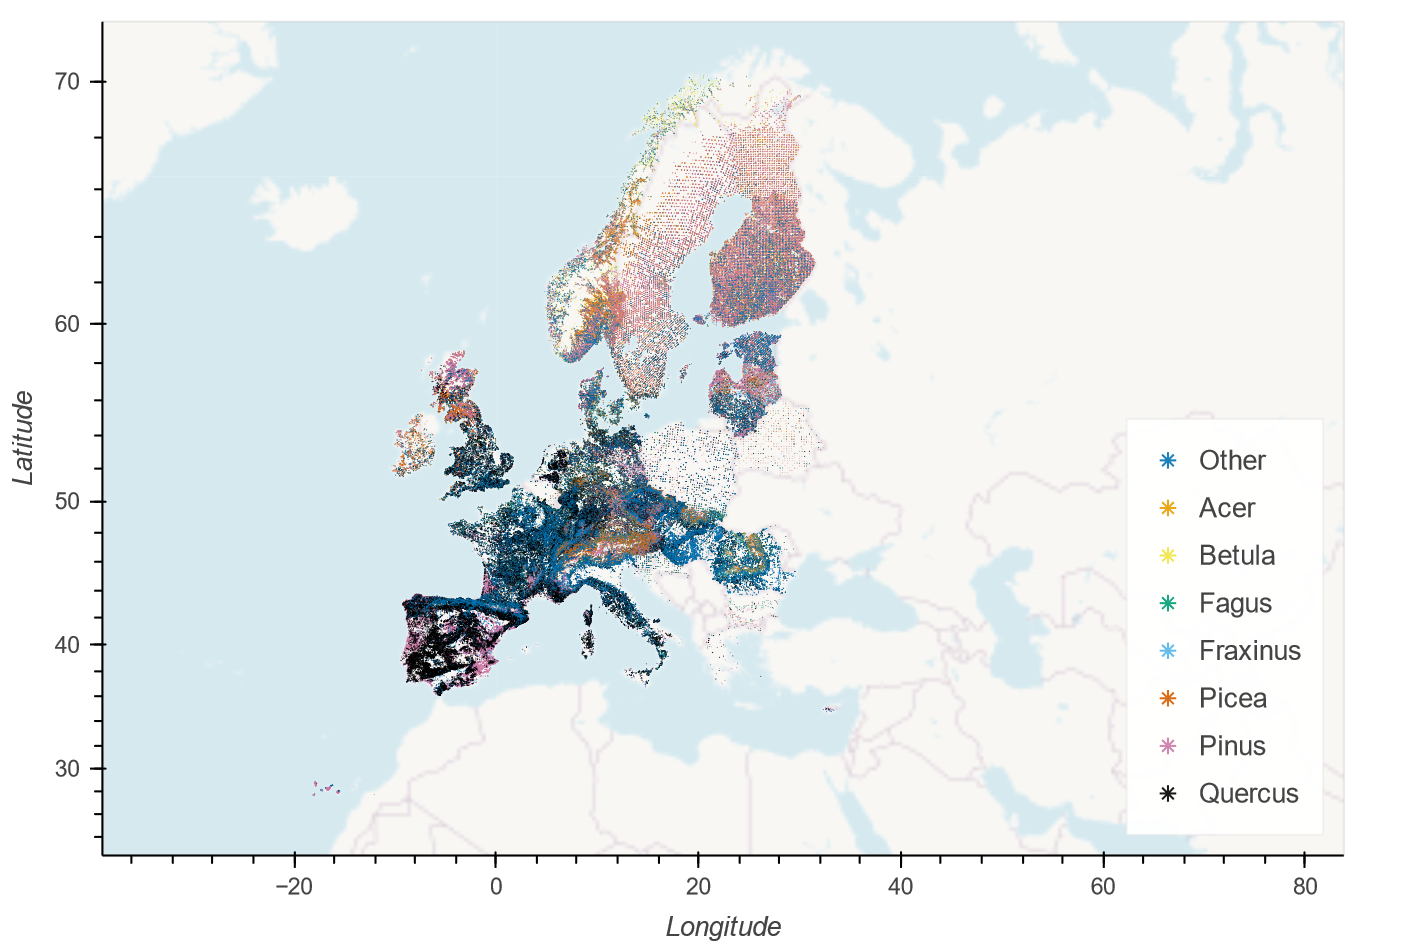
\includegraphics[width=0.98\linewidth]{figures/figures_labels/genus_cutoff_map.png}
    \caption{Map of the most common tree genera in EU-Forest.}
    \label{fig:genus_cutoff_map}
\end{figure}

EU-Forest is a dataset containing tree species and genera for nearly $250,000$ locations across Europe. Each plot is 1\,km\,×\,1\,km and may contain multiple tree species and genera. Fig.\,\ref{fig:genus_cutoff_map} shows the distribution of tree genera in the EU-Forest dataset across 21 European countries. In this figure, the label 'Other' is an umbrella class for 70 tree genera with less than 20,000 occurrences each.

Using the EU-Forest dataset to train a CNN classifier of tree genera with Sentinel-2 data offers several significant advantages. Firstly, the dataset's high spatial resolution enables fine-grained 
analysis of tree species distribution, which enhances the accuracy of the classifier. Its comprehensive coverage across Europe, including diverse forest types and geographical areas, allows the model to learn from a wide variety of environments and tree genera. The rich occurrence data provides detailed information on tree species, aiding in precise identification and classification.

\begin{figure}[!thb]
    \centering

    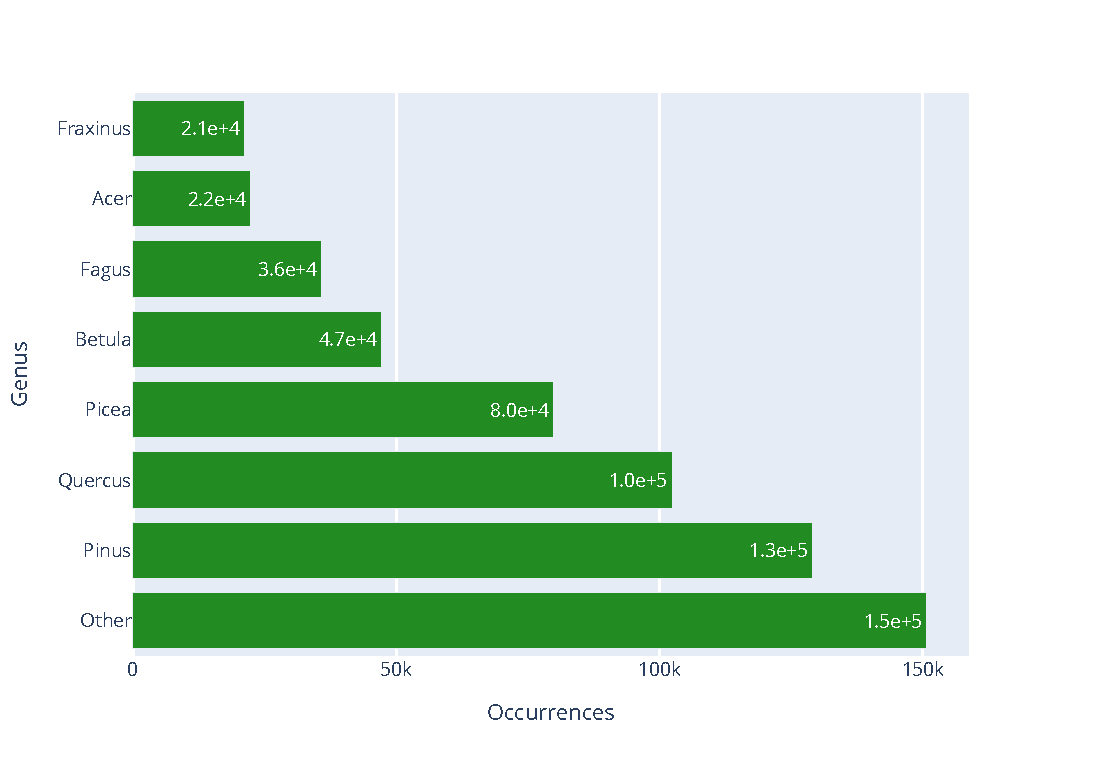
\includegraphics[width=0.48\linewidth, trim={0 0 2cm 0}]{figures/figures_labels/genus_cutoff.pdf}
    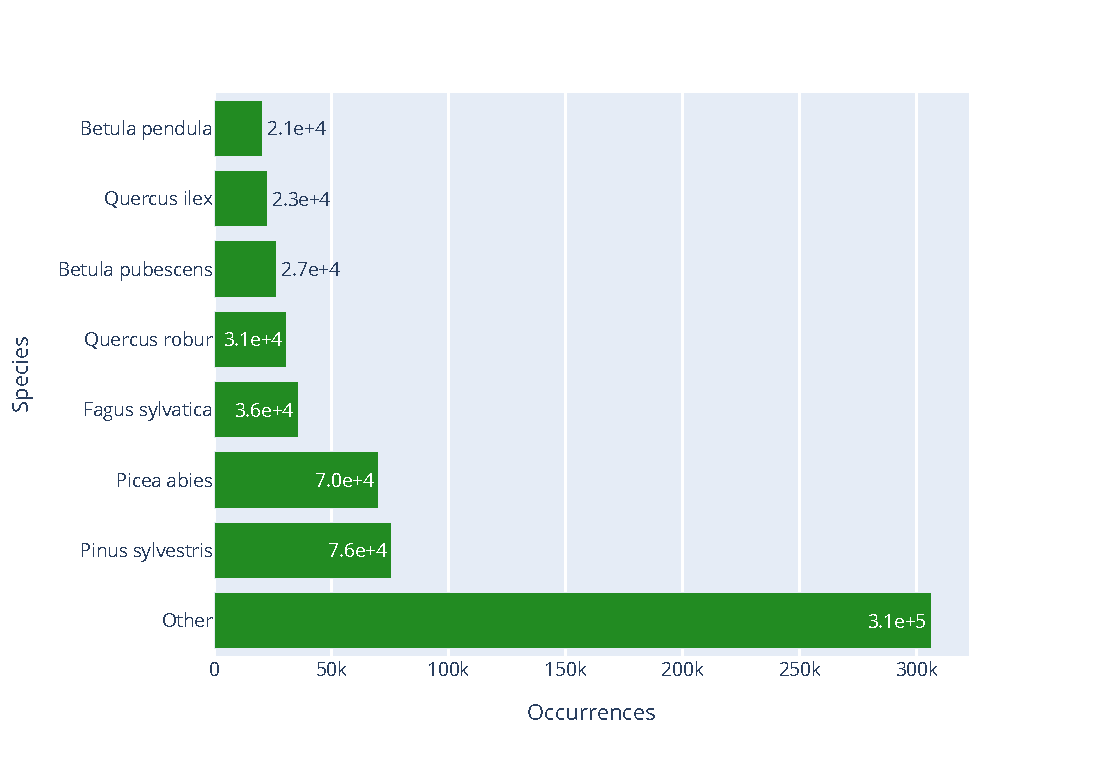
\includegraphics[width=0.48\linewidth, trim={0 0 2cm 0}]{figures/figures_labels/species_cutoff.pdf}

    \caption{Distribution of genera (left) and species (right) in EU-Forest.}
    \label{fig:cutoff_barplots}
\end{figure}

Integration with Sentinel-2 satellite data, which provides high-resolution multispectral images, allows for a robust model that leverages both ground-truth data and spectral information. The dataset, being relatively recent, offers a contemporary snapshot of forest conditions, ensuring that the trained model is relevant to current ecological and environmental conditions. 

The plots in Fig.\,\ref{fig:cutoff_barplots} underscore the prevalence of certain genera and species in European forests, providing valuable insights for training a CNN classifier. The dominance of specific genera and species in the dataset can enhance the classifier's ability to accurately identify and classify tree types when combined with Sentinel-2 data.

\begin{figure}[!thb]
    \centering

    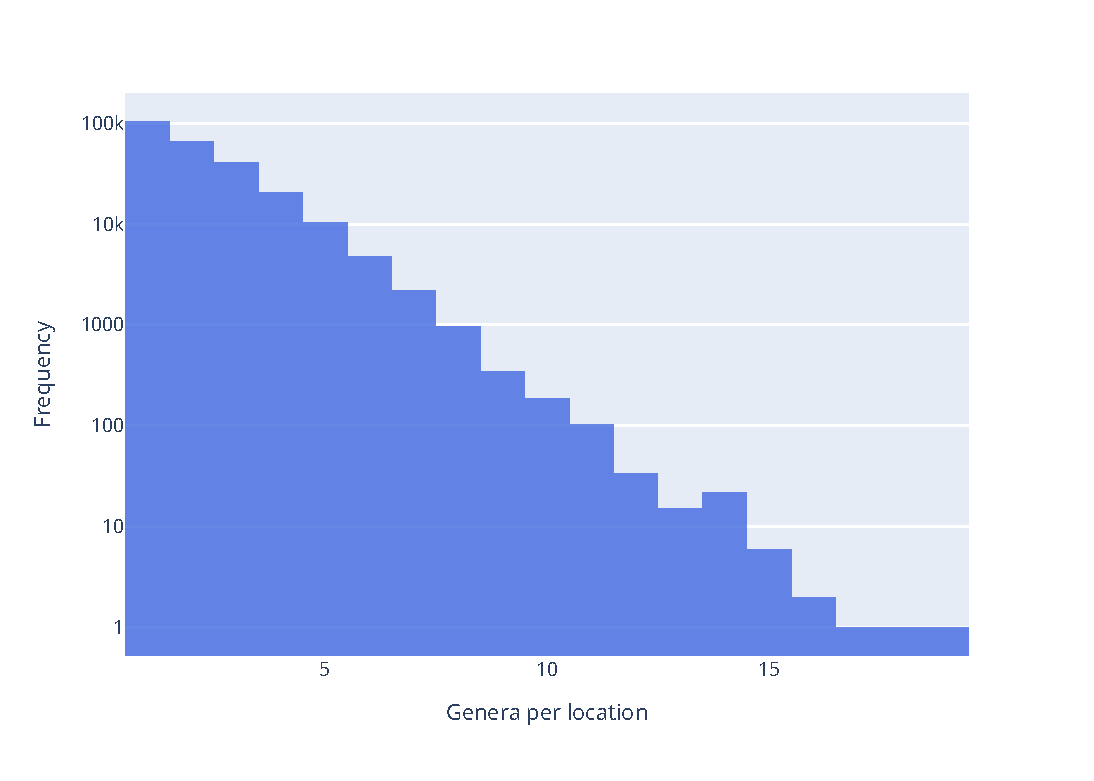
\includegraphics[width=0.48\linewidth, trim={0 0 2cm 0}]{figures/figures_labels/grouped_genus.pdf}%
    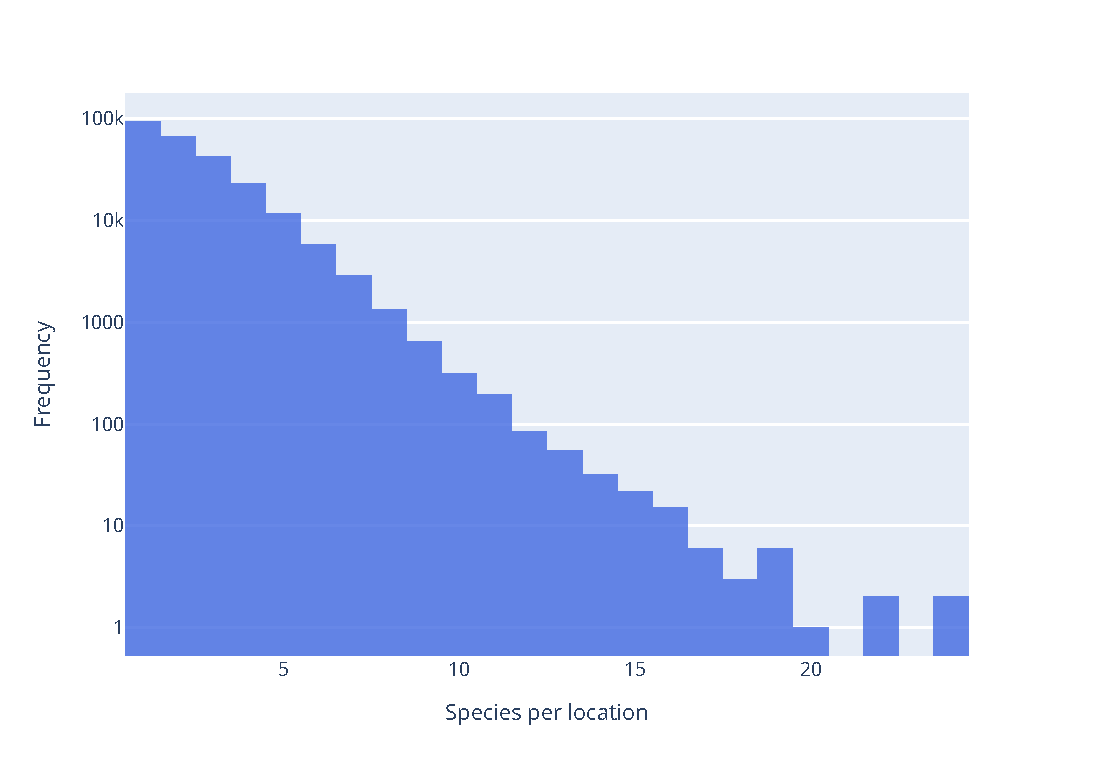
\includegraphics[width=0.48\linewidth, trim={0 0 2cm 0}]{figures/figures_labels/grouped_species.pdf}

    \caption{Distribution of genera (left) and species (right) per location.}
    \label{fig:grouped_histograms}
\end{figure}
 
The plots in Fig.\,\ref{fig:grouped_histograms} reveal a common pattern in biodiversity studies: most locations are characterized by a limited number of dominant genera and species, with a smaller number of locations exhibiting higher diversity. This pattern is important for training a CNN classifier, as it indicates that the classifier will often encounter locations with limited genera and species. However, it must also be capable of handling the less common, more diverse locations. The high-frequency, low-diversity areas will likely dominate the training process, influencing the classifier's ability to generalize across different forest types.

\section{Sentinel-2 Features}

\begin{figure}[ht]
    \centering
    \href{https://sentinels.copernicus.eu/documents/247904/4180891/Sentinel-2-infographic.pdf}
    {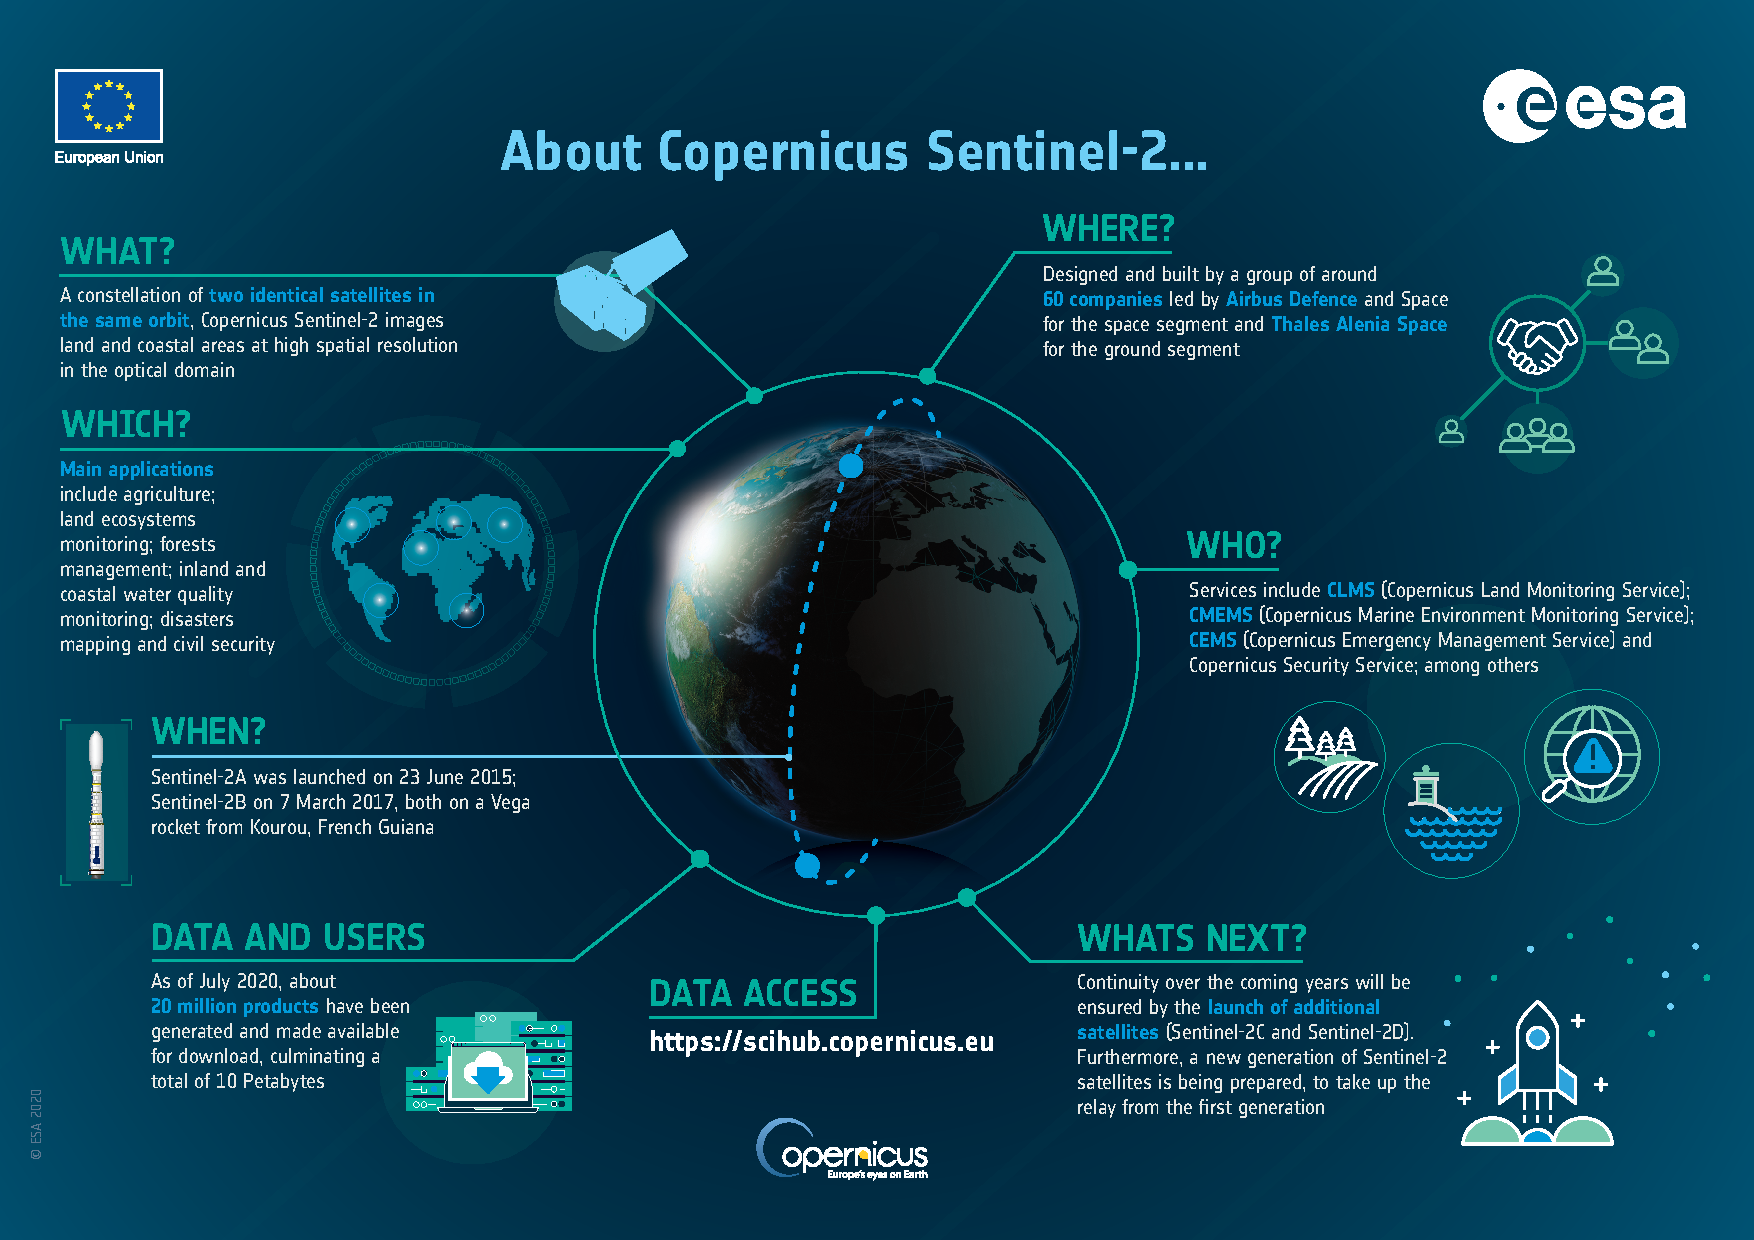
\includegraphics[width=0.98\linewidth]{figures/figures_sentinel/Sentinel-2-infographic.pdf}}
    \caption{Sentinel-2 mission infographic. It highlights important facts and achievements of the mission. Courtesy of \href{https://sentinels.copernicus.eu/web/sentinel/missions/sentinel-2}{ESA}.
    }
    \label{fig:sentinel2_info}
\end{figure}

Using Sentinel-2, Fig.\,\ref{fig:sentinel2_info}, specifically the 10-meter and 20-meter resolution bands, for training a CNN classifier of tree genera offers several significant advantages. Sentinel-2 provides high-resolution imagery with these bands capturing detailed spatial information essential for precise classification tasks.

The 10-meter resolution bands include visible red, green, and blue (RGB) wavelengths, as well as near-infrared (NIR) wavelengths, which are essential for assessing vegetation health and differentiating tree genera based on their reflectance properties. The 20-meter resolution bands encompass the red-edge, shortwave infrared (SWIR), and additional near-infrared regions, which enhance the classifier's ability to distinguish between tree genera by capturing subtle variations in spectral signatures. For subsequent analysis, the 20-meter bands were resampled to match the 10-meter resolution.

The multispectral imaging capability of Sentinel-2, with these selected bands, allows for detailed analysis and precise classification of tree genera. Each genus reflects and absorbs light differently across these wavelengths, providing rich data for the classifier to learn from and accurately identify tree types.

Moreover, Sentinel-2 has a frequent revisit time, with satellites passing over the same area every 5 days at the equator. This frequent update cycle is crucial for handling cloud cover, as it increases the likelihood of acquiring cloud-free images, ensuring that the classifier is trained on clear and usable data.

\begin{figure}[!thb]
    \centering

    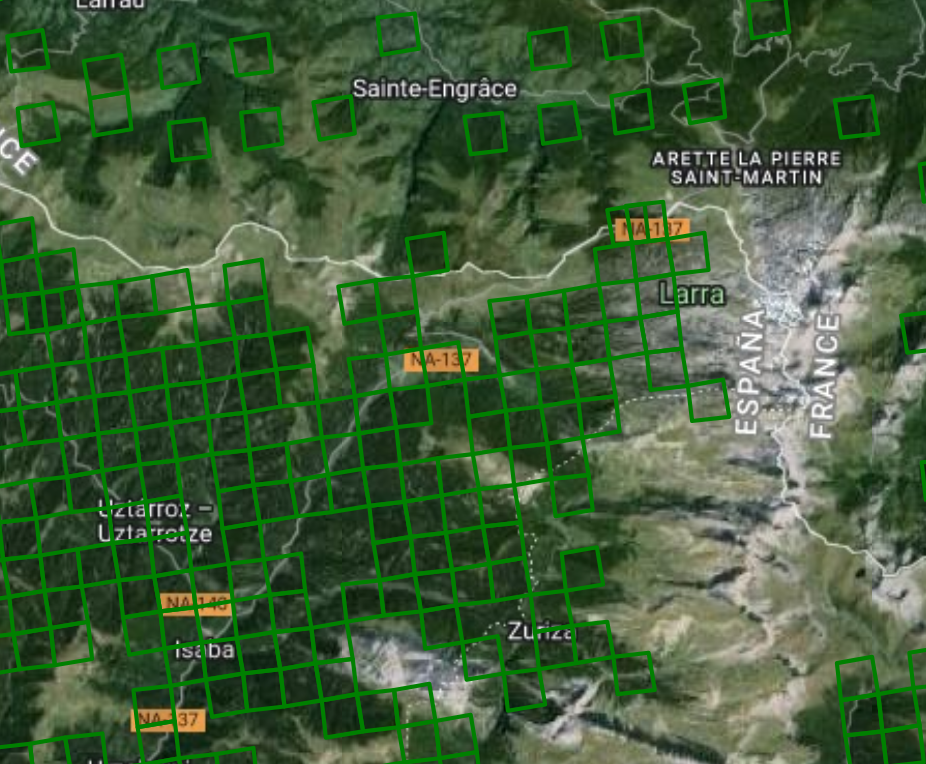
\includegraphics[width=0.48\linewidth]{figures/figures_sentinel/sample_area_earth.png}
    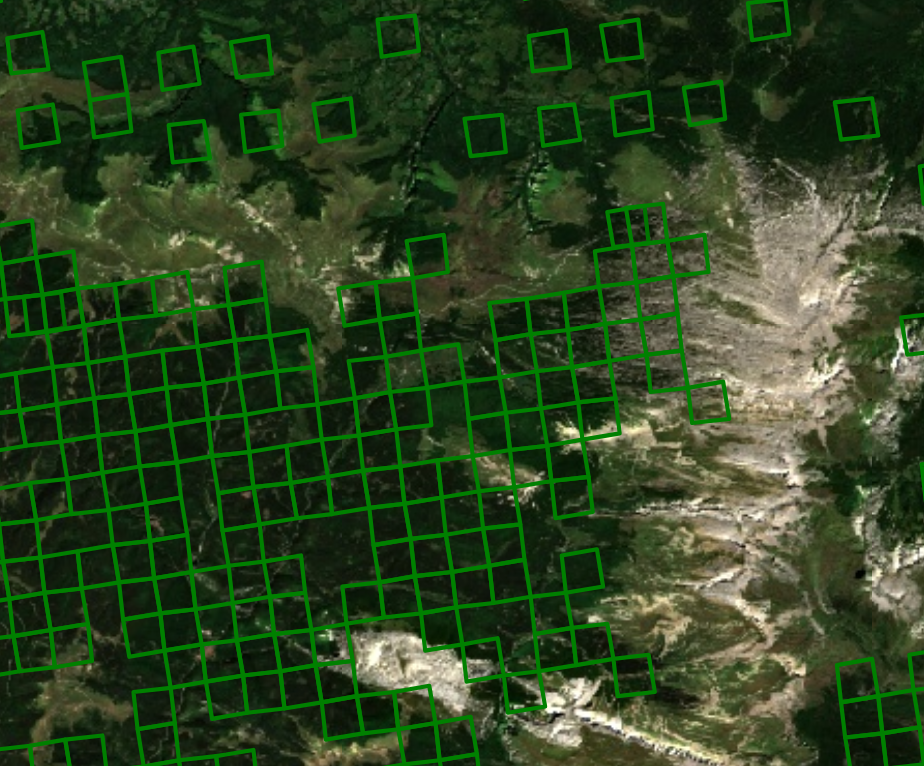
\includegraphics[width=0.48\linewidth]{figures/figures_sentinel/sample_area_sentinel.png}

    \caption{Multiple sample locations overlaid on Google Earth (left) and Sentinel-2 (right) images.}
    \label{fig:label_sample_area}
\end{figure}

Sentinel-2 also offers extensive geographical coverage, capturing large areas in each image. This comprehensive coverage is essential for training classifiers intended for wide-ranging applications across different forest types and regions, and it supports the development of global models for tree genus classification.

Additionally, Sentinel-2 data is freely available through the European Space Agency's Copernicus program and Google Earth Engine. This open access eliminates budget constraints, ensuring high-quality satellite data is accessible for research and operational purposes.

\begin{figure}[!thb]
    \centering

    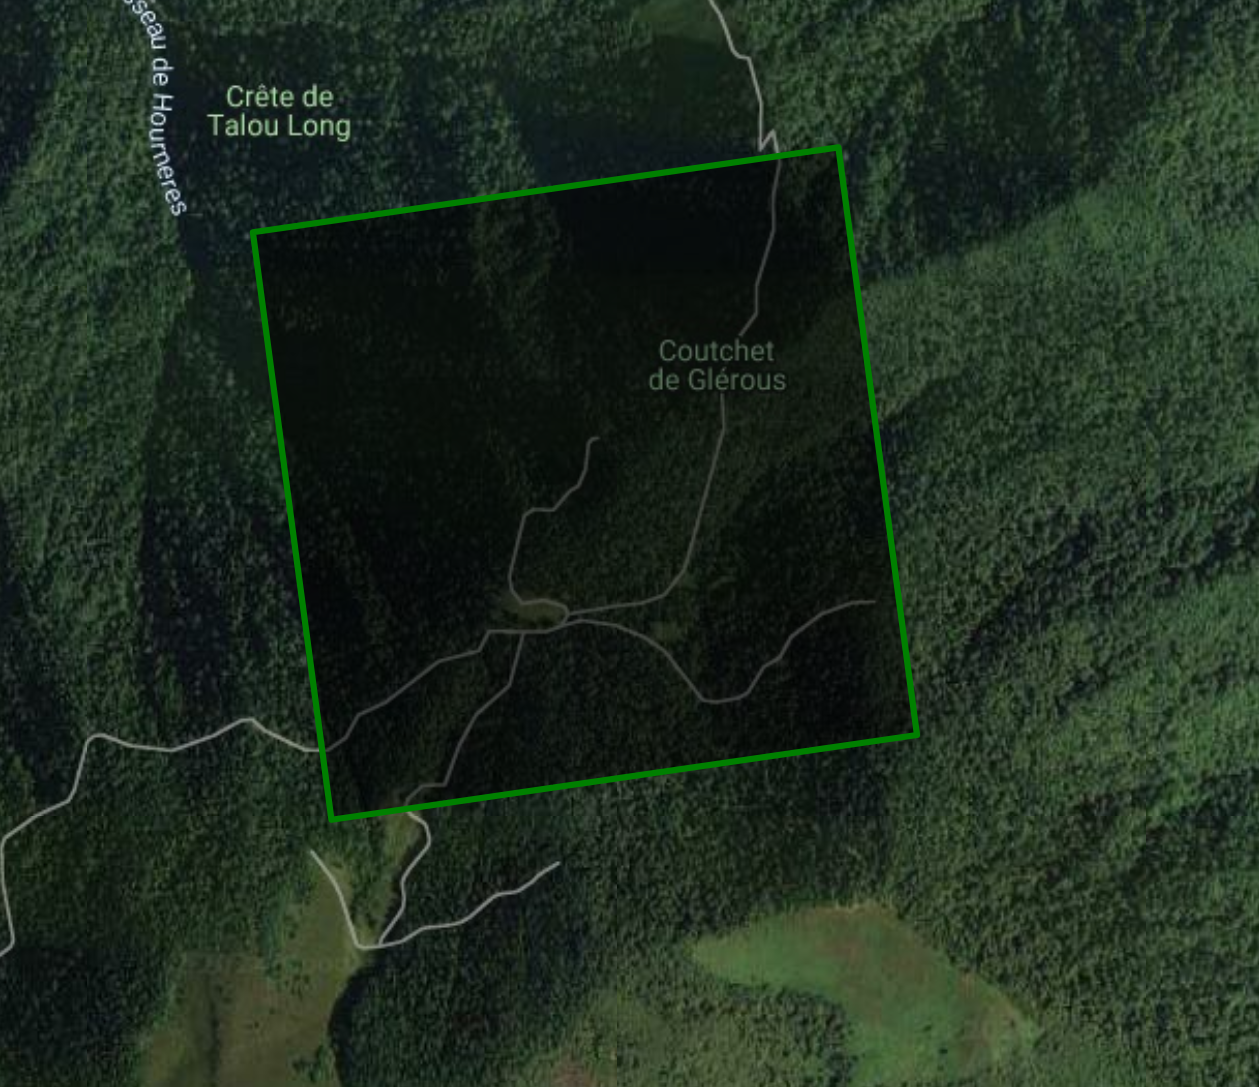
\includegraphics[width=0.48\linewidth]{figures/figures_sentinel/sample_earth.png}
    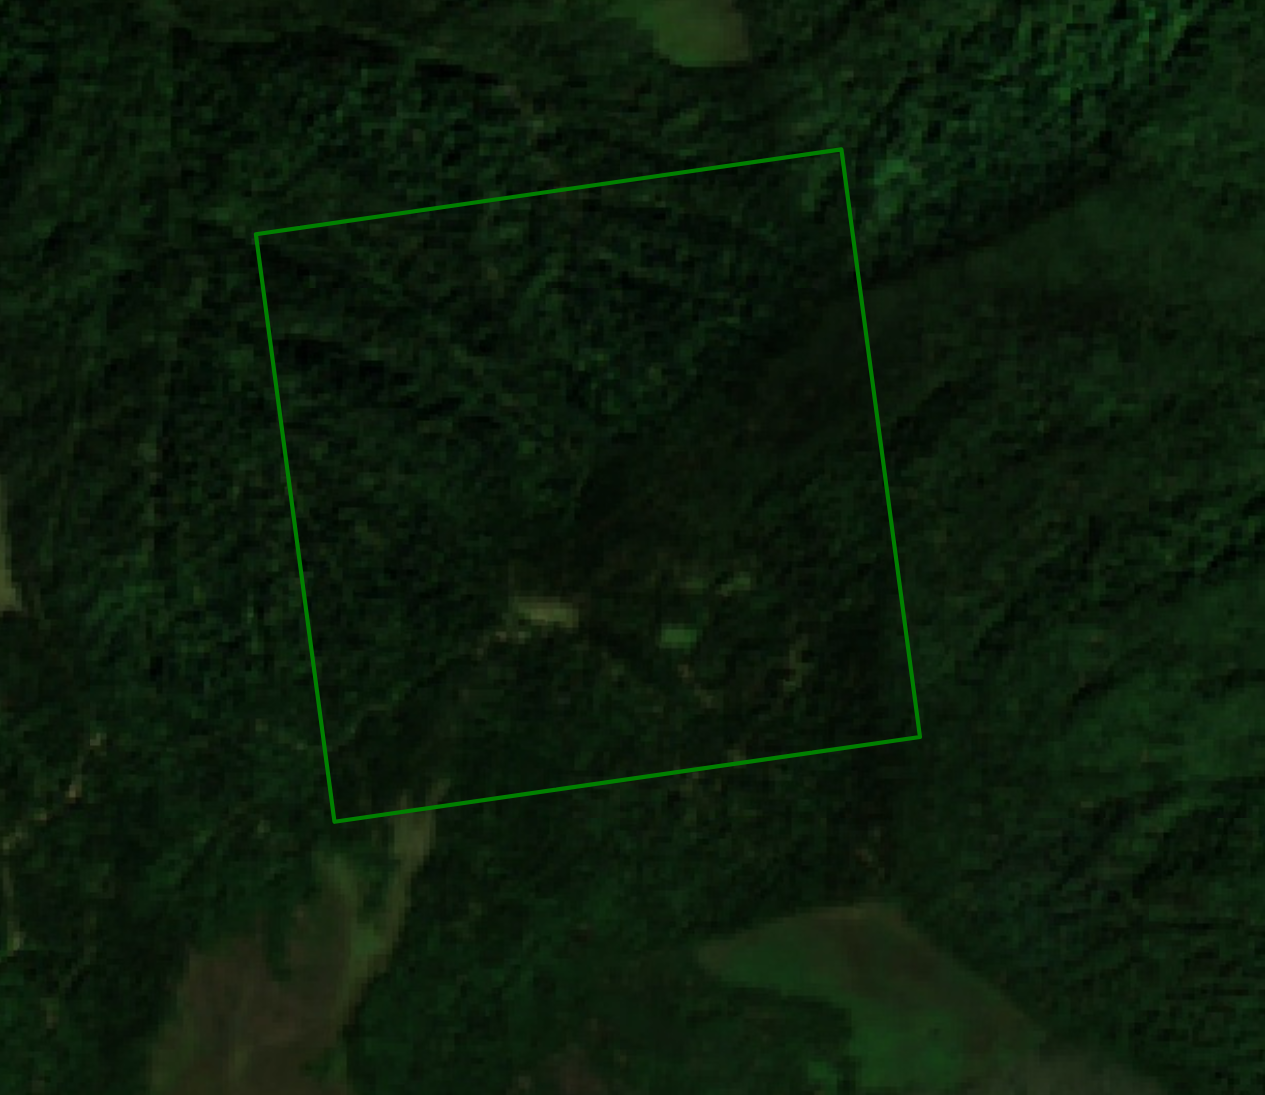
\includegraphics[width=0.48\linewidth]{figures/figures_sentinel/sample_sentinel.png}

    \caption{Sample location overlaid on Google Earth (left) and Sentinel-2 (right) images.}
    \label{fig:label_sample}
\end{figure}

Figs.\,\ref{fig:label_sample_area} and \ref{fig:label_sample} illustrate the integration of high-resolution geographical context with Sentinel-2 satellite data for detailed environmental analysis. The grid overlay in the images represents areas for data collection and analysis. The left images provide a more detailed geographical context, while the right images show how Sentinel-2 bands B2, B3, and B4 (blue, green, and red respectively) are structured and utilized for spectral analysis.


\begin{figure}[ht]
    \centering
    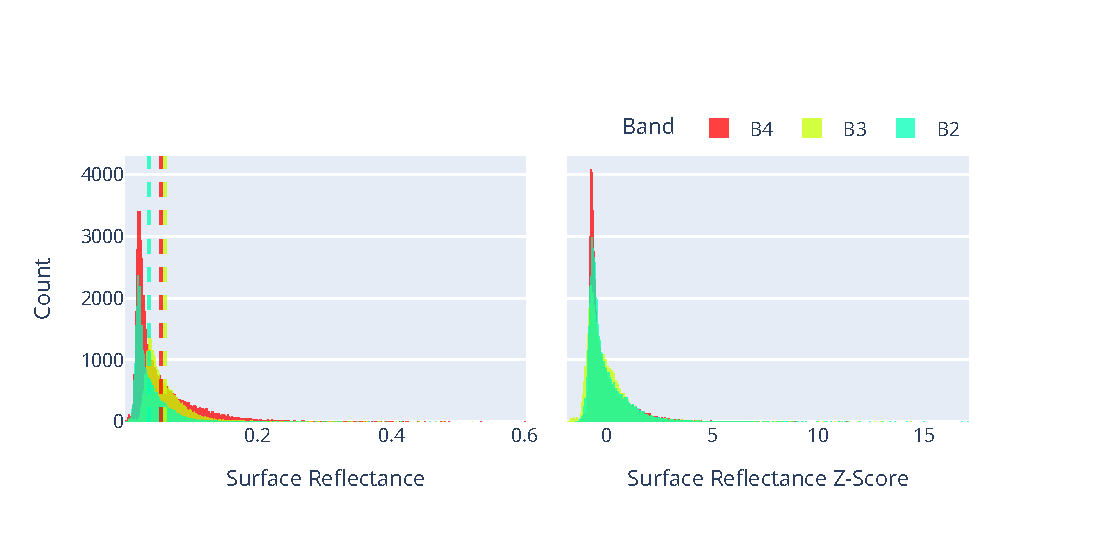
\includegraphics[width=0.98\linewidth, trim={15pt 25pt 10pt 50pt}, clip]{figures/figures_features/bgr_hist.pdf}
    \caption{Distributions for surface reflectance (left), including a sample means as a dotted line, and z-score normalization (right) for RGB bands.}
    \label{fig:bgr_hist}
\end{figure}

\begin{figure}[ht]
    \centering
    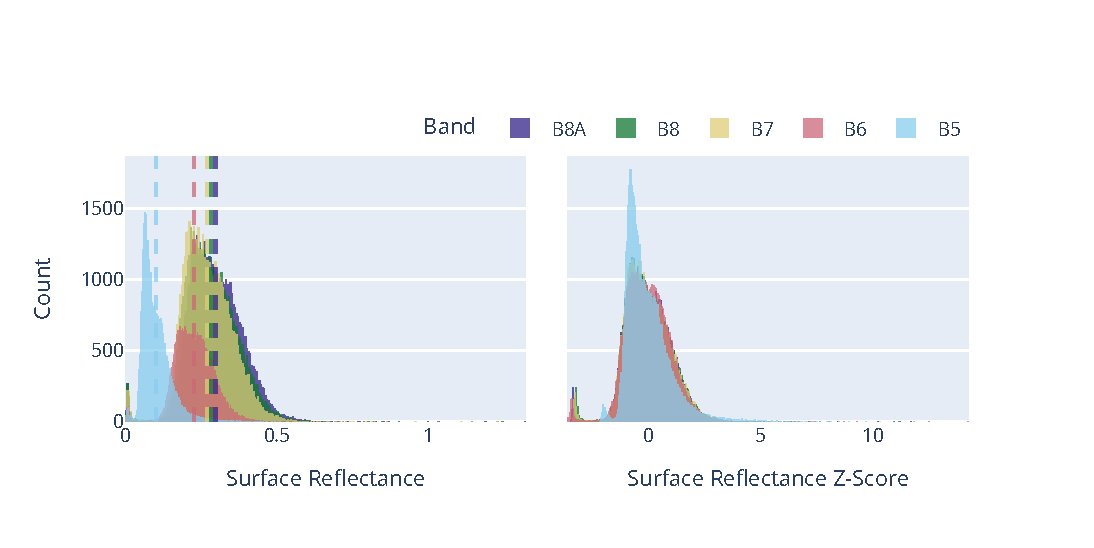
\includegraphics[width=0.98\linewidth, trim={15pt 25pt 10pt 50pt}, clip]{figures/figures_features/nir_hist.pdf}
    \caption{Distributions for surface reflectance (left), including a sample means as a dotted line, and z-score normalization (right) for NIR bands.}
    \label{fig:nir_hist}
\end{figure}

\begin{figure}[ht]
    \centering
    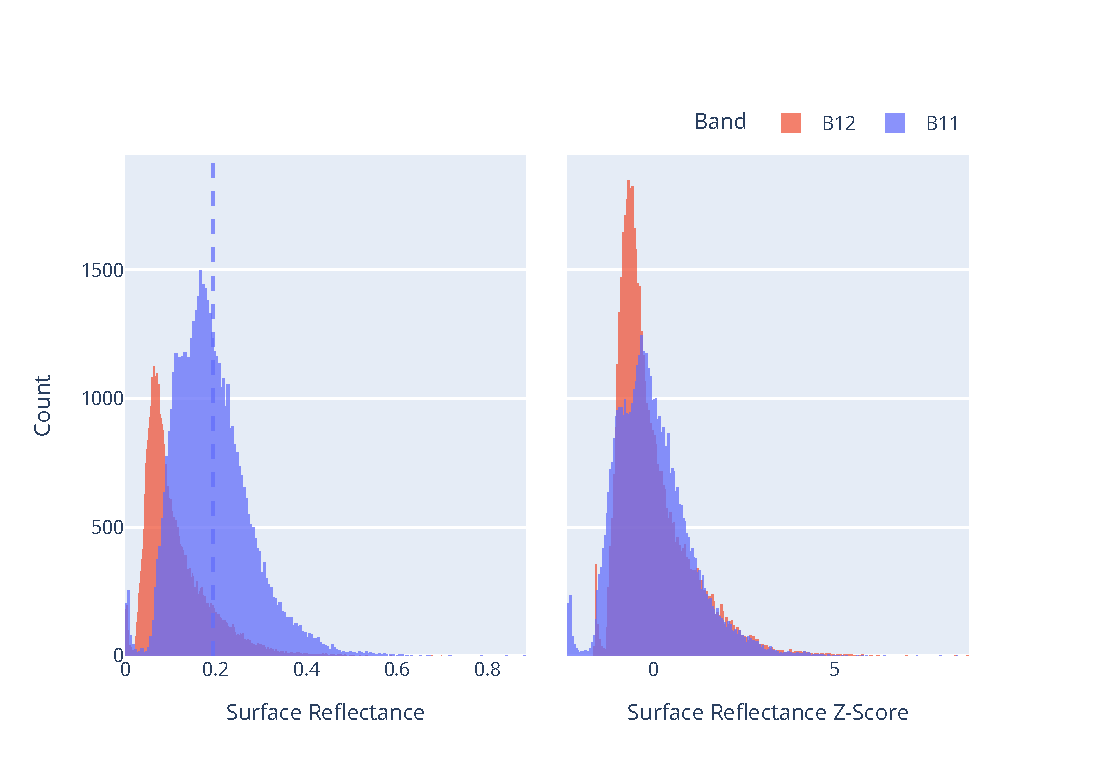
\includegraphics[width=0.98\linewidth, trim={15pt 25pt 10pt 50pt}, clip]{figures/figures_features/swir_hist.pdf}
    \caption{Distributions for surface reflectance (left), including a sample means as a dotted line, and z-score normalization (right) for SWIR bands.}
    \label{fig:swir_hist}
\end{figure}

Figs.\,\ref{fig:bgr_hist}, \ref{fig:nir_hist}, and\,\ref{fig:swir_hist} provide a detailed look at the distribution of surface reflectance values and their z-scores for various Sentinel-2 spectral bands, a normalization method which is crucial for many classification tasks using CNNs. These figures use medians taken over the summer months (June, July, and August) between 2017, 2018, and 2019.

Fig.\,\ref{fig:bgr_hist} shows that the reflectance values for the bands B2, B3, and B4 generally follow a log-normal distribution. The z-scores for these bands peak near zero, demonstrating that the reflectance values have been normalized effectively. This normalization is essential for ensuring that the values from different bands are on the same scale, which is particularly important when using CNN for classification.

Fig.\,\ref{fig:nir_hist} presents the distribution for the NIR bands B5, B6, B7, B8, and B8A. The reflectance values for these bands display a central tendency, with a significant number of pixels having values around the mean. The z-score distributions, peaking near zero, indicate successful normalization of the reflectance values. Normalizing the data in this way ensures that the CNN can process and compare these values more effectively, enhancing the model's ability to classify different types of tree genera accurately.

Fig.\,\ref{fig:swir_hist} shows histograms for the SWIR bands B11 and B12. The bands display a similar pattern, with the majority of reflectance values clustering on the left of the mean and tailing off to the right of the mean. The z-scores for these bands also peak at zero, confirming that the data has been normalized successfully. 


\begin{figure}[ht]
    \centering
    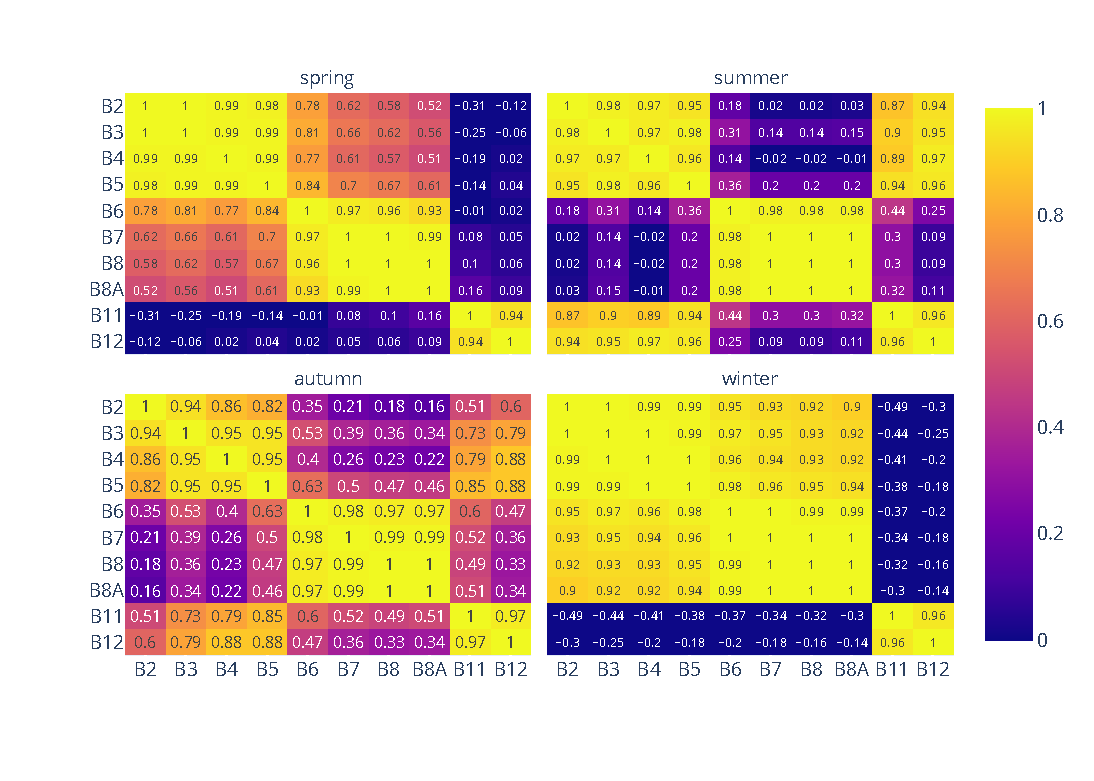
\includegraphics[width=0.98\linewidth, trim={40pt 40pt 10pt 30pt}, clip]{figures/figures_features/season_correlation.pdf}
    \caption{Seasonal Sentinel-2 band correlations.}
    \label{fig:season_correlation}
\end{figure}

The correlations among different spectral bands of Sentinel-2 data across seasons, as depicted in the correlation matrices in Fig.\,\ref{fig:season_correlation}, highlight significant patterns that are useful for tree genus classification. All plots show the Pearson's correlation coefficients between various bands, providing insights into how these relationships change with the seasons.

During winter, all bands in NIR and RGB groups show very strong correlations with each other. These high correlations, often close to 1, indicate that the spectral responses of these bands are highly similar during this season. This consistency is likely due to the uniform reflectance properties of vegetation and the ground cover in winter. This strong correlation is beneficial for tree genus classification as it suggests that the data from these bands can be reliably used to distinguish tree genera based on their reflectance characteristics, or lack thereof, in winter.

In spring, the correlations remain high within the NIR and RGB groups but to a slightly lesser degree compared to winter. The correlation between these two groups starts to decrease, reflecting the changes in vegetation as new growth begins. This seasonal variation provides additional information that can be leveraged to improve the classification models, as the differences in reflectance between the bands become more pronounced.

During summer and autumn, while there are still strong correlations within the NIR and RGB groups, the correlation between these groups is notably lower. This reduced correlation can be attributed to the varying phenological stages of the trees, including differences in leaf development and moisture content. These seasonal changes affect the reflectance properties differently in the NIR and RGB bands. The distinct spectral responses during these seasons offer complementary information that can enhance the classification of tree genera by providing a more diverse set of data points that capture the variability in tree characteristics.

Overall, the varying correlations across seasons underscore the robustness of using Sentinel-2 data for tree genus classification. Normalizing the data using z-scores is crucial as it standardizes the values across different bands, ensuring they are on the same scale. This is particularly important for CNNs, which are sensitive to the relative magnitudes of input data. By bringing the bands to a comparable scale, z-score normalization enhances the model's ability to process and accurately compare the multi-band data, leading to more reliable and precise classification results.

\section{Copernicus DEM GLO-30}

Integrating the Copernicus Global 30\,m Digital Elevation Model (DEM) data into the classification model can significantly enhance its performance for tree genus classification. Elevation data provides critical information about the terrain, which influences various ecological factors such as temperature, moisture availability, and soil type. These factors, in turn, affect vegetation types and distribution. The 30\,m resolution of the DEM is particularly well-suited for this purpose, as it offers a fine enough scale to capture relevant topographic features while being broad enough to complement the 10\,m and 20\,m resolutions of Sentinel-2 data. This synergy allows the model to better understand the environmental context of each location, leading to more accurate predictions. For example, certain tree genera may be more prevalent at specific elevation ranges due to their adaptation to particular climatic conditions or soil properties. Therefore, integrating elevation data can help in distinguishing between tree genera that occupy different ecological niches.

Fig.\,\ref{fig:elevation_hist} presents the distribution of elevation values in meters, as well as the z-scores, which standardize these values. The elevation values range from 0 to around 2500 meters, with most data points clustered below 500 meters. This suggests that the majority of the study area is relatively low-lying. Standardizing elevation values using z-scores is beneficial for integrating elevation data with spectral data, as it ensures that elevation values are on a comparable scale to the reflectance values from Sentinel-2 bands. 

\begin{figure}[ht]
    \centering
    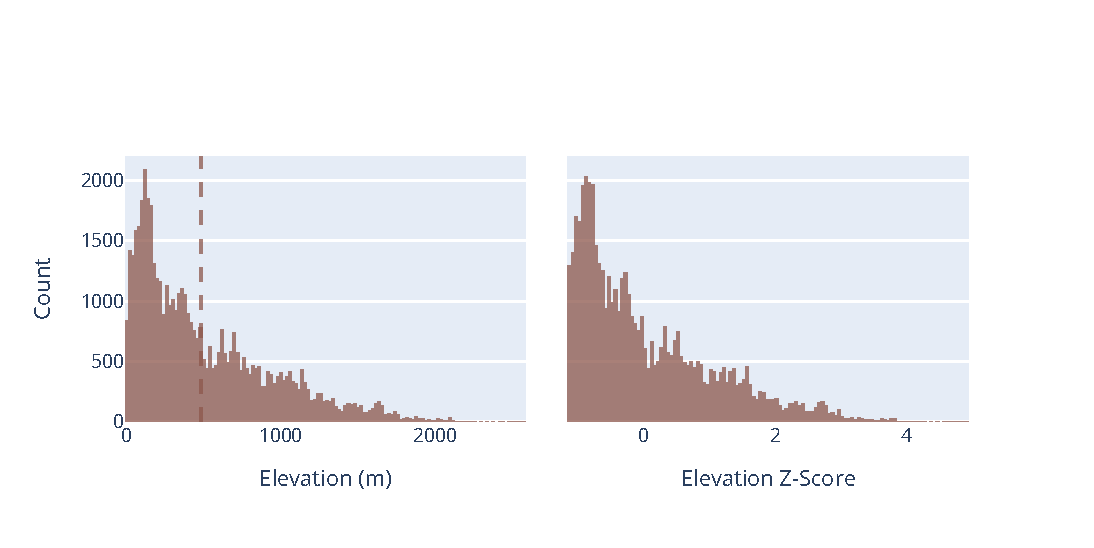
\includegraphics[width=0.98\linewidth, trim={15pt 25pt 10pt 50pt}, clip]{figures/figures_features/elevation_hist.pdf}
    \caption{Distributions for elevation (left), including a sample means as a dotted line, 
    and z-score normalization (right) for the Copernicus DEM GLO-30 dataset.}
    \label{fig:elevation_hist}
\end{figure}

\section{SoilGrids}

The SoilGrids dataset provides global soil information at a spatial resolution of 250 meters and incorporates quantified spatial uncertainty. It includes key soil properties such as organic carbon content, pH, sand, silt, and clay percentages, bulk density, cation exchange capacity, and more. These data are derived from machine learning models trained on extensive soil sample databases and environmental covariates.

Integrating SoilGrids data into the tree genus classification model can significantly enhance its performance. Soil properties profoundly influence vegetation types and distribution, as different tree genera have specific soil requirements and preferences. For instance, soil pH, nutrient content, and texture can determine the suitability of a habitat for particular tree species. By incorporating detailed soil composition data, the model can better understand the environmental context, leading to more accurate predictions of tree genera. This integration helps to account for the ecological niche of each genus, improving the robustness and precision of the classification.

\begin{figure}[ht]
    \centering
    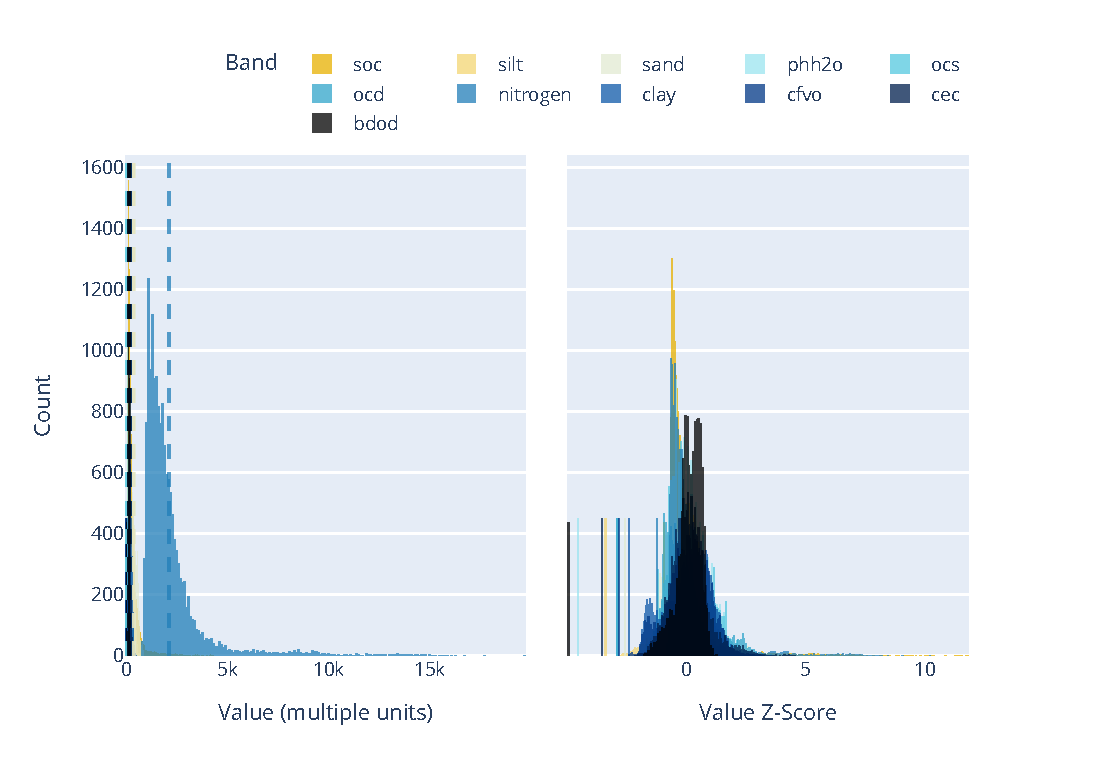
\includegraphics[width=0.98\linewidth, trim={15pt 25pt 10pt 20pt}, clip]{figures/figures_features/soil_hist.pdf}
    \caption{Distributions for soil properties (left), including a sample means as a dotted line, and z-score normalization (right) for the SoilGrids dataset.}
    \label{fig:soil_hist}
\end{figure}

Fig.\,\ref{fig:soil_hist} displays the distribution of various soil properties present in the SoilGrids dataset. The x-axis represents the value of these properties in multiple units, while the y-axis represents the count of observations. Additionally, the z-score distribution is shown to standardize these values.

The distribution of soil properties varies, reflecting the diversity of soil types across the study area. The z-score distribution standardizes these values, bringing them onto a common scale, which is essential for integrating soil data with spectral and elevation data in the classification model.

\section{Summary}

While the integration of high-resolution Sentinel-2 imagery with EU-Forest data, Copernicus DEM elevation information, and SoilGrids soil properties provided a comprehensive dataset, the improvement in model accuracy was marginal. This suggests that, for the task of tree genus classification, the spectral information from Sentinel-2 may be sufficiently robust on its own. However, these additional datasets might still offer value in specific contexts or could enhance model performance in more complex classification tasks or in areas with greater environmental variability.